\documentclass[a4paper, 10pt, conference]{ieeeconf}

\usepackage[dvipsnames]{xcolor}

\usepackage{times}
\usepackage{graphicx}
\usepackage{amssymb}
\usepackage{amsmath}
\usepackage{breakurl}
\def\UrlBreaks{\do\/\do-}
\usepackage{url,hyperref}
\usepackage{algorithm}
\usepackage{algorithmic}
\usepackage[labelfont={bf},font=small]{caption}
\usepackage[none]{hyphenat}
\usepackage{mathtools, cuted}
\usepackage[noadjust, nobreak]{cite}
\usepackage{tabularx}
\newcolumntype{Y}{>{\centering\arraybackslash}X}
\usepackage{afterpage}
\usepackage{stfloats}
\usepackage{comment}
\usepackage{xcolor,colortbl}

\newcommand{\specialcell}[2][c]{%
  \begin{tabular}[#1]{@{}c@{}}#2\end{tabular}}

\title{\LARGE \bf
A Gateway to Astronomical Image Processing: Rubin Observatory Science Pipelines on AWS
}

\author{
    Dino Bektesevic$^1$, Andrew Connolly$^1$ \\
    Department of Astronomy, University of Washington \\ Email: dinob@uw.edu, ajc@uw.edu
    }

\begin{document}


\maketitle


%%%%%%%%%%%%%%%%%%%%%%%%%%%%%%%%%%%%%%%%%%%%%%%%%%%%%%%%%%%%%%%%%%%%%%%%%%%%%%%%
\begin{abstract}

The Legacy Survey of Space and Time\footnote{\url{www.lsst.org}} (LSST) is a 10-year astronomical survey due to start operations in 2022 that will image half the sky every three nights. LSST will produce approximately 20TB of raw data per night, which be calibrated and analyzed in almost real time.  Given the volume of LSST data, the traditional subset-download-process paradigm of data reprocessing faces significant challenges. We describe a gateway for astronomical science that would enable astronomers to analyze images and catalogs at scale. In this first step we focus on executing the LSST's Science Pipelines, a collection of image and catalog processing algorithms, on Amazon Web Services (AWS). We describe the workflow management system (Pegasus\cite{}) and HTCondor\cite{}) used to execute a data processing pipelines and manage compute resources, the interface to this gateway (Jupyterlab \cite{}), and the performance, scalability and cost of deploying this system in the cloud.
\end{abstract}

%%%%%%%%%%%%%%%%%%%%%%%%%%%%%%%%%%%%%%%%%%%%%%%%%%%%%%%%%%%%%%%%%%%%%%%%%%%%%%%%
\section{INTRODUCTION}

The currently pervasive model of sub-selecting, transferring to local compute resources and then reprocessing data was successful in context of past astronomical sky-surveys such as such as Sloan Digital Sky Survey\cite{York2000} (SDSS) because technological developments and pricing made acquiring sufficient local compute resource affordable. With a new generation sky surveys such as the LSST delivering an order of magnitude more data this subset-download-process paradigm is no longer viable. We describe a new approach, utilizing the elastic capabilities of cloud compute resources to enable users to scale their analyses to 100TB+ data sets and to access these resources through a simple and intuitive gateway.

%Drawing on lessons learned from previous surveys and in order to facilitate scientific discovery LSST reduces the raw data into multiple different, smaller in volume, science products. LSST also offers 10\% of their compute resources for use to in-collaboration scientists. Even though this approach mitigates a lot of associated problems it does not do away with the need to process pixel level data. At LSST's data volumes however, considering even a relatively small subset of data will amount to a large dataset. For example, over the lifetime of the survey a 1\% random subset of the total data still constitutes a 5 PB large dataset - three the size of PanSTARRS, the largest to-date astronomical image dataset. To reprocess even such small subsets of total data, significant computing resources, and subsequently significant initial investments, are required.

Our initial objective is to provide astronomers with an interface and tools that allow them to process an entire nights worth of LSST data in hours and to do so at a reasonable cost. As a first step towards such a gateway we focus on image data reduction pipelines. Such pipelines  consist of a series of sequential steps that calibrate the data, detect all sources, potentially cross reference them to previously known sources and measure their properties (or features). Additionally, images covering the same area of the sky are stacked (co-added) in order to increase the signal-to-noise of the resulting coadd, and subtracted  in order to detect sources that have moved or changed brightness. A typical input and output of such a pipeline is shown on figure-\ref{fig:raw2calexp} where a raw image has been calibrated to remove instrumental effects. Many existing data reduction pipelines are conglomerations of bespoke code written for specific applications, leaving the astronomical image data reduction landscape in a fragmented state where usually only the larger sky surveys offer tools to scientists for data reduction and often where these tools are difficult to set-up and use or do not scale to petabyte scale surveys.

%On face value, enabling reprocessing of LSST data using the LSST data reduction pipelines, would at least guarantee repeatability and reproducibility. But 
By design, the LSST data reduction pipelines can support many different instruments and cameras on a range of different telescopes including  Dark Energy Camera (DECam, \cite{DECam}), Hyper-Suprime Cam (HSC, \cite{HSC}), Sloand Digital Sky Survey (SDSS, \cite{SDSS}, and Canada-France-Hawaii Telescope (CFHT, \cite{CFHT}). Exposing the Science Pipelines functionality through a common interface would pave-the-way towards standardization of data reduction pipelines, enabling state-of-the-art astronomical data processing algorithms as well as the definition and execution of custom analysis pipelines for bespoke data sets. The need for scalability and the ability to share the resulting data across a range of communities naturally leads to a cloud compute model whether commercial or academic. 

%There are many different software solutions that perform these tasks but rarely can they be applied at scale or %perform all of the described processing steps. 

\begin{figure}[htb]
\centering
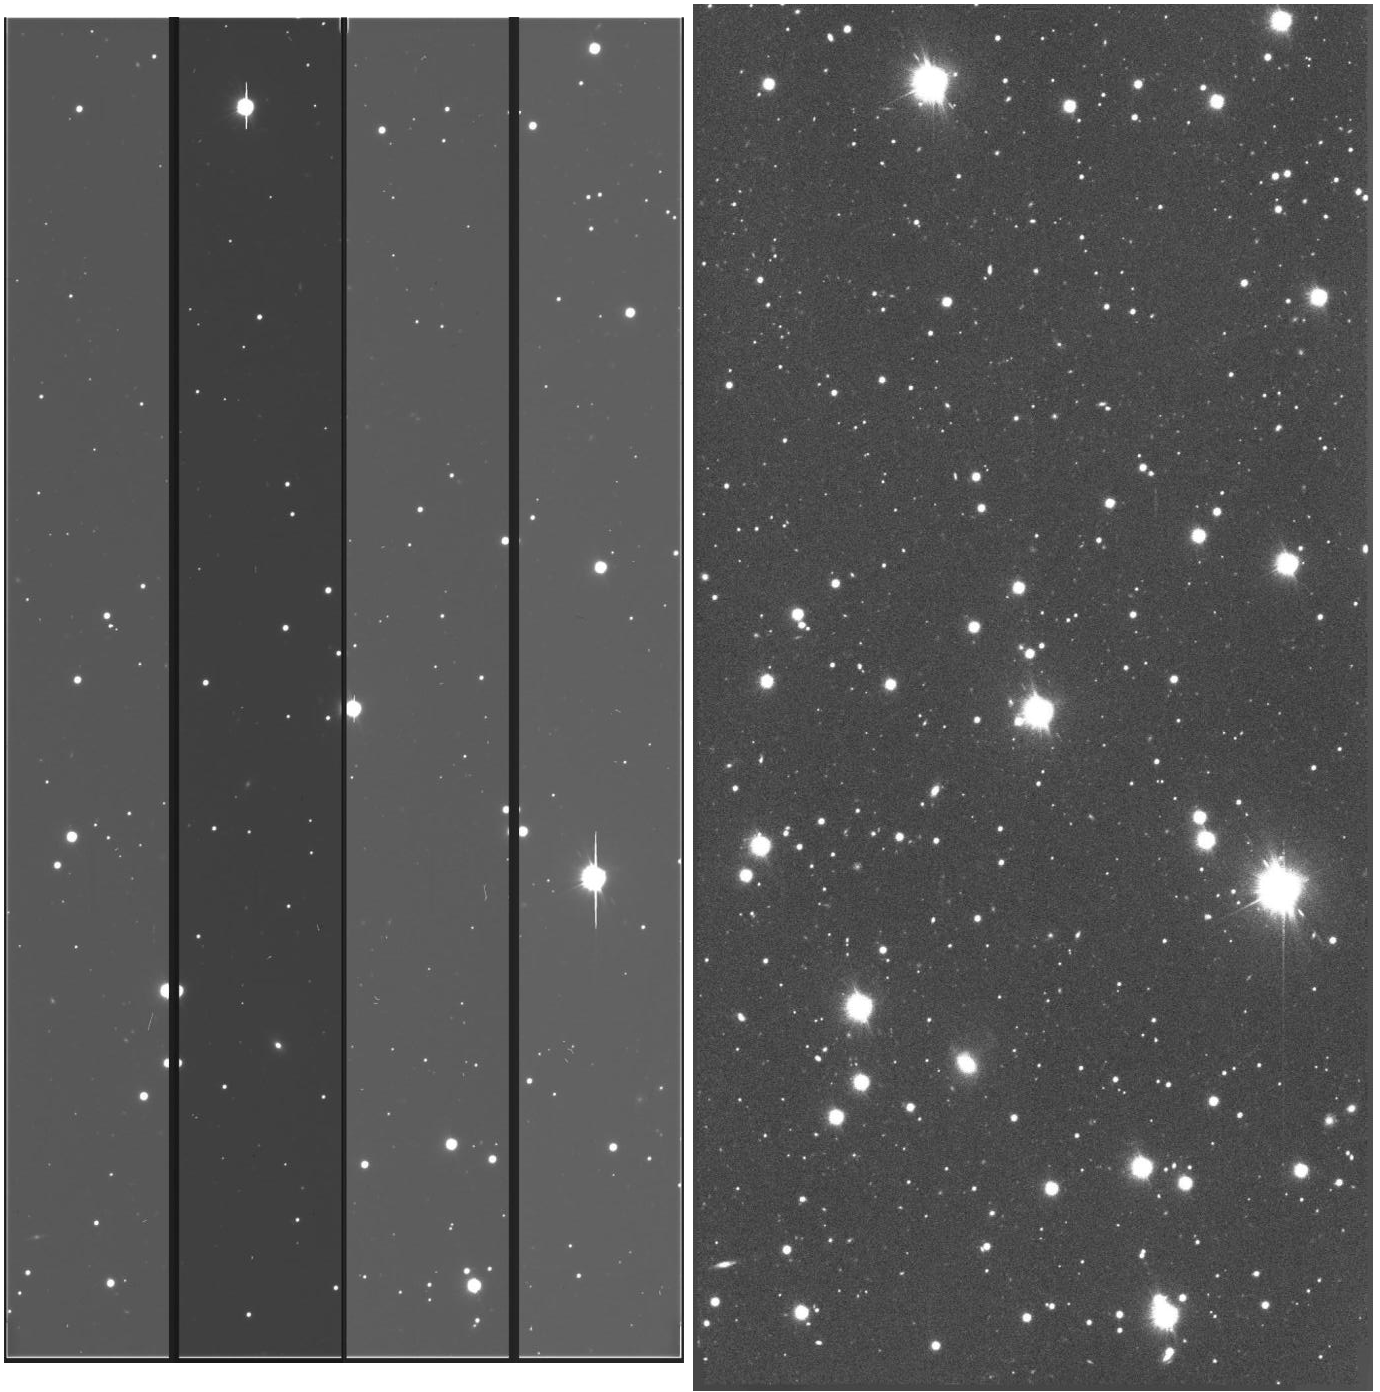
\includegraphics[angle=-90,width=0.8\columnwidth]{figures/raw2calexp.png}
\caption{A raw, uncalibrated image from the HSC (top) and the resulting calibrated exposure after processing with the LSST data management stack (bottom). The images are not the same size because calibration adjusts for the optic distorsion of the instrument.}
\label{fig:raw2calexp}
\end{figure}




%%%%%%%%%%%%%%%%%%%%%%%%%%%%%%%%%%%%%%%%%%%%%%%%%%%%%%%%%%%%%%%%%%%%%%%%%%%%%%%%
\section{Technology Stack}
\label{sec:techstack}

While cloud technology has been adopted  quickly by some scientific communities, see \cite{NatLang}, \cite{HEPCloud} or \cite{IceCube}, and the IT industry, it's adoption by the Astronomical community has been slow. Legacy code is typically designed with the assumption that data exists locally or that there exists a globally accessible file system, that the processing is some form of batch processing, and that the system is in general not state agnostic. While it is possible to create similar systems in the cloud, the cloud infrastructure is generally not conducive to such a design and is more oriented towards shared-nothing filesystems \cite{sharednothing}, containerization \cite{containerization} and near-data processing architectures. 

%To achieve our goals we have to resort to new additions to the legacy codes and tools and to add functionality where it is missing. These tools and code changes are described in mode details in sections \ref{subsec:scipipe} and \ref{subsec:pegasuscondor}, while section \ref{subsec:aws} describes the used cloud services

%As aforementioned, astronomical data reduction pipeline consists of many individual steps. Steps, generally speaking, need to be ordered as subsequent ones depend on data products of previous one and each step can require significantly different resources than the previous steps. 

In the following sections we describe the enhancement of the code base to address these issues. To achieve scalability, while maintaining  resource allocation flexibility, we use a workflow manager, to which we describe and submit a workflow, and a resource manager, through which we procure required resources. The workflow description is provided by the LSST Science Pipelines and consists of individual jobs targeting single datasets, the description of each job's required resources as well as the interdependence of different jobs in the workflow. 
\begin{figure}[htb]
\centering
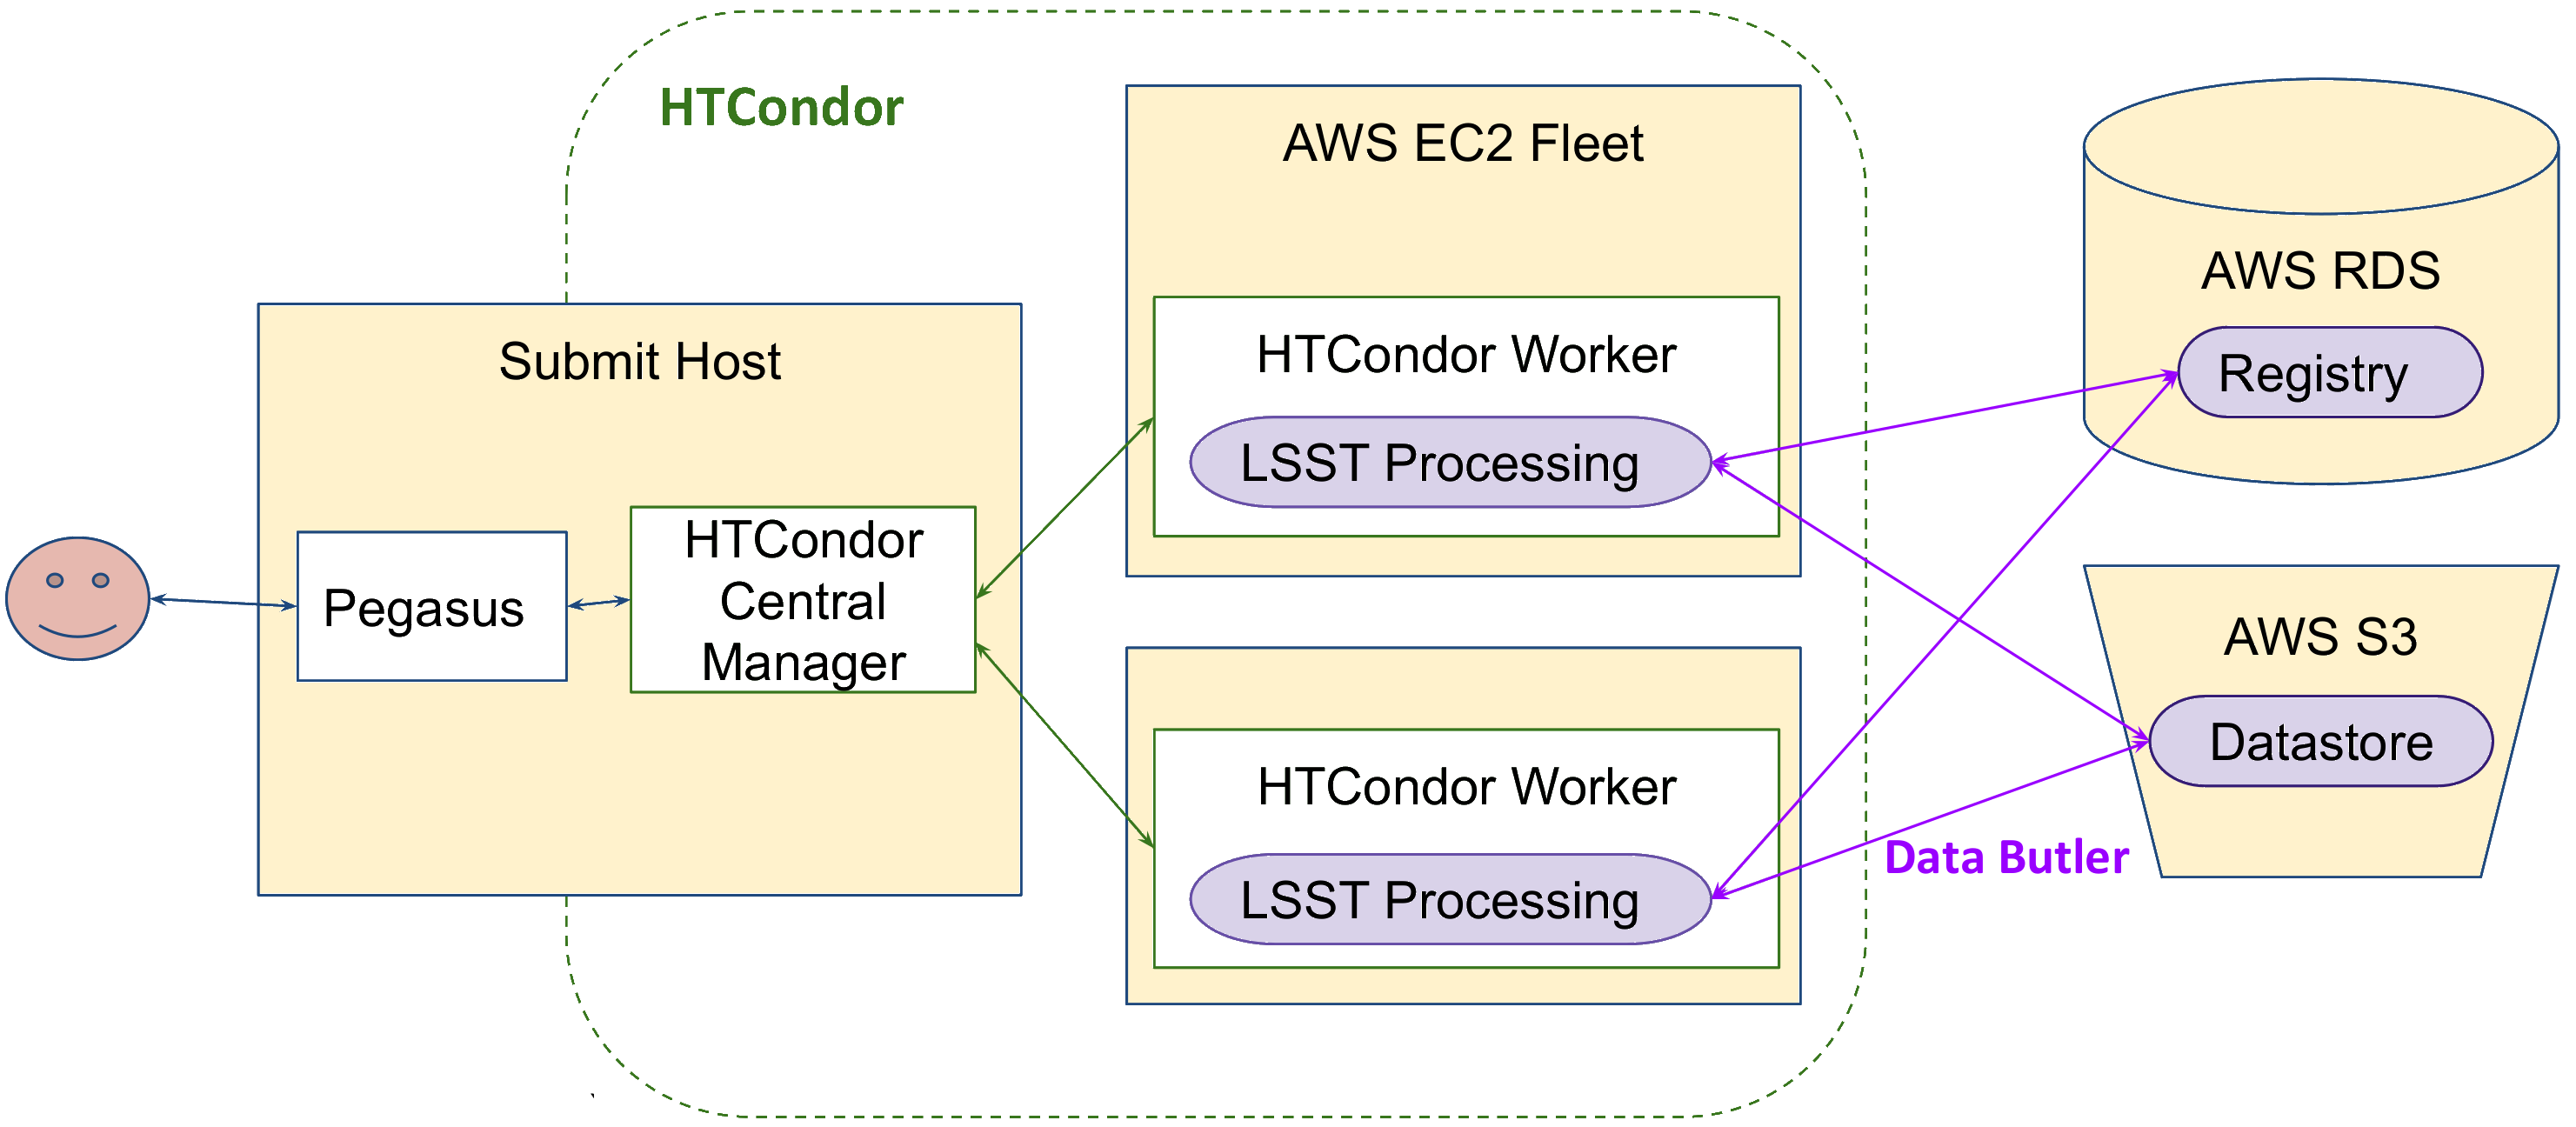
\includegraphics[width=\columnwidth]{figures/workflow.png}
\caption{The workflow stack for the LSST cloud compute engine. A user, leftmost, gains access to the master node which contains the LSST Science Pipelines, Pegasus and HTCondor. Using the Science Pipelines the user creates a Quantum Graph of a workflow they want to run. Users procures compute resources, workers, using HTCondor and submits the workflow to Pegasus. As Quanta are executed on the workers the persisted data is written to the Datastore, an S3 Bucket, and to a Registry, an RDS PostgreSQL database. Workers either deallocate themselves after being IDLE for an user set amount of time or terminate after a user set maximum time is reached. The persisted data remains accessible to the user from the master and other locations as well.}
\label{fig:techstack}
\end{figure}
Scaling is achieved by scheduling as many parallel jobs of the same type as resources allow. When the compute cluster is under-subscribed, such as when the resource requirements are very high or when there are not enough same-type jobs to schedule simultaneously, the resource manager will deallocate the idle resources for cost optimization. New resources can also be allocated and dynamically added to the cluster when resource requirements of the jobs change. 

These actions are undertaken from a persistent "master" node with users interacting with the components of our system through a JupyterLab interface. 

\begin{figure}[htb]
\centering
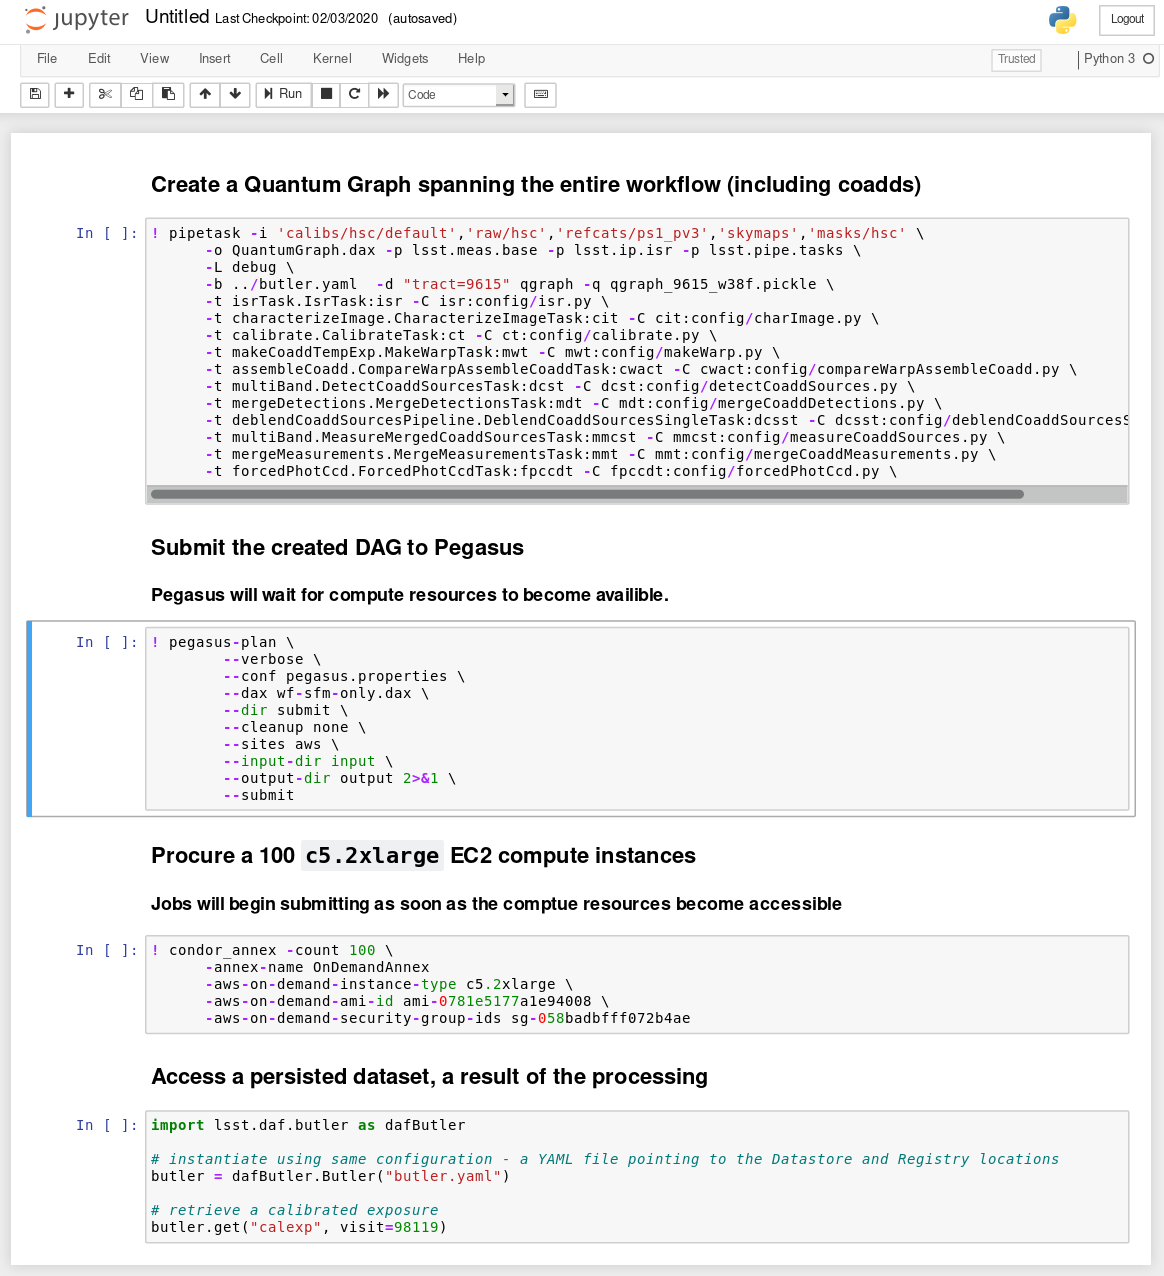
\includegraphics[width=\columnwidth]{figures/JupyterNotebookFakery.png}
\caption{An example of Jupyter Notebook interface. }
\label{fig:techstack}
\end{figure}

The LSST science pipelines represent the state-of-the-art in astronomical data reduction. They consist of variety of configurable Tasks that can be chained into a pipeline. Such a pipeline is described by a directed acyclic graph (DAG) called a QuantumGraph (\cite{dmtn055}). Quantum Graph consists of quanta, which is a task applied to an individual dataset. The science pipelines enable processing of optical and near-infrared astronomical data from a single visit (instrument signature removal, characterization, calibration, coaddition, forced photometry etc) to overarching tasks such as joint calibration that constrains astrometric and photometric measurements across multiple different visits. 

Tasks themselves are agnostic to file formats and locations of the data. The input-output (IO) and provenance is tracked through a middleware component called the Data Butler. The main purpose of the Data Butler is to isolate the end user from file organization, filetypes and related file access mechanisms by exposing datasets as, mostly, Python objects. Datasets are referred to by their unique IDs, or a set of identifying references. Data Butler uses a registry to resolve the dataset references and resolves the location, file format and the Python object/type of the files stored in a datastore.

The registry is almost always backed by an SQL database and the datastore is usually backed by a shared filesystem. The data butler has been modified to be cloud aware with a registry and datastore capable of utilizing AWS resources (\cite{dmtn114} and \cite{dmtn137}).

\href{https://research.cs.wisc.edu/htcondor}{HTCondor} \cite{Thain:2005:HTCondor} provides distributed job parallelization and is a powerful batch system for high throughput computing (HTC). HTCondor Annex allows HTCondor deployment on cloud resources via acquisition of cloud compute resources external to an existing HTCondor pool. A pool can have multiple annexes, and each annex manages its own lifecycle. Unused compute resources are automatically deallocated after a user-set time spent idling. 

\href{https://pegasus.isi.edu/}{Pegasus} \cite{Deelman:2015:Pegasus} is a workflow management system built on top of HTCondor.
It provides command line and API interfaces for scientists to write an abstract workflow independent of the underlying computing infrastructure. Pegasus workflows are expressed as DAGs and Quantum Graphs are interpretable by Pegasus. Pegasus comes with various tools for data management, f.e. log transfers, and supports different execution strategies by grouping jobs within or across nodes of a DAG.

To facilitate running Science Pipelines we implemented an \href{https://aws.amazon.com/s3/}{Simple Storage Service (S3)} back-end for the Datastore. S3 is an object storage that allows massive amounts of unstructured data, where each object typically is identified by a globally unique identifier. We also implemented a PostgreSQL backed Registry off-the-shelf support for spatial primitives needed for querying astronomical data (\cite{PostGIS}). The PostgresSQL database is managed through the \href{https://aws.amazon.com/rds/}{Relational Database Service (RDS)} service.
Elastic Compute Cloud (EC2) is used to acquire compute resources.  In the following sections we evaluate the cost and performance of various instance types.

%%%%%%%%%%%%%%%%%%%%%%%%%%%%%%%%%%%%%%%%%%%%%%%%%%%%%%%%%%%%%%%%%%%%%%%%%%%%%%%%
\section{Example Workflow}

The example workflow is based off of the well understood, well characterized HSC Release Candidate dataset\footnote{\url{https://jira.lsstcorp.org/browse/DM-11345}} tract 9516. This dataset is reprocessed using Rubin Obs. compute resources every two weeks in order to characterize the scientific validity and performance of the algorithms as they are being developed. There are 6787 instrument signature removal (ISR) jobs. ISR removes image features that are the result of instrument flaws. Characterization consists of modeling the background, point spread function (PSF), repairing cosmic ray traces, detecting and measuring bright sources.
There are, again, 6787 characterize tasks in the workflow. Finally the calibration tasks detect all sources on the images and measure the astrometric and photometric properties of these sources. The workflow is shown on figure \ref{fig:demo-workflow}.

\begin{figure}[htb]
\centering
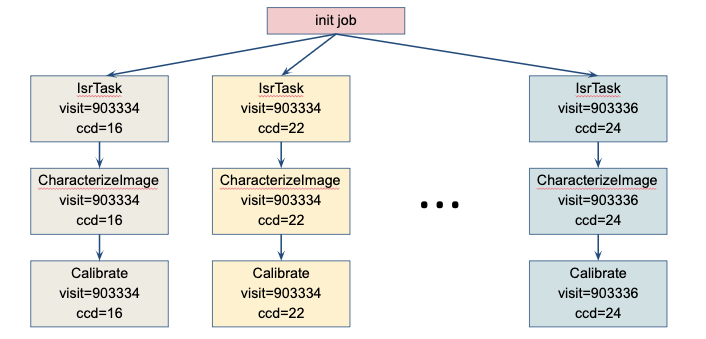
\includegraphics[width=\columnwidth]{figures/demo-workflow.png}
\caption{Example workflow on which performance and scalability was tested. Initialization job sets the Registry by creating any new output collections or dataset type entries. Processing consists of instrument signature removal, characterization and calibration. These are ordered jobs for each image but processing a set of images is an embarrassingly parallel problem.}
\label{fig:demo-workflow}
\end{figure}

The total size of the input data is 0.2TB and the size of output data is approximately 2.7TB. In number of visits processed this represents $\sim$11\% of the number of observations per night from the Rubin Observatory. Figure \ref{fig:raw2calexp.png} shows the comparison between the raw input image and the output data, a calibrated exposure.


\section{Performance, scalability and cost}

The example workflow was evaluated for multiple different instance types and instance sizes. The tests were performed on on-demand and on spot instance types. The wall time is the cumulative value of execution times of all Tasks in the Quantum Graph, including the scheduling and execution overhead. Results are summarized in table \ref{fig:costWallTime}.  

The full processing takes approximately ??? hours for a canonical 25 instance configuration. Of this  
initialization  takes on average 22-30 minutes. We exclude this from all results because this initialization is required to run only once per each new output collection.
%This time should not be considered when scaling the execution times to larger datasets because the initialization job is required to run only once per each new output collection and thus would not be run again for any subsequent processing steps or would it be run multiple times if the DAG contained more Tasks. 

%Pegasus and HTCondor offer comprehensive and very detailed control over scheduling and execution of jobs. However, as discussed in section \ref{sec:techstack}, these tools were designed and optimized primarily with a more classical HPC computing architectures in mind and the adopted default values for many parameters that control every aspect of execution reflect that. 

We consider two approaches: (1) A baseline where we implement that LSST science pipelines as configure for a grid-like system (i.e.\ the architecture for which they were initially designed). In this implementation there are nearly 6GB in pickled configuration files (Quanta) and log files. As we discus below this presents a very large IO bottleneck since without a shared file-system these jobs rely on ftp, sftp, rsync and other internet transfer protocols to transfer between the master and workers.

%stage-in and out phases of the workflow execution. Namely Quantum Graph nodes, i.e. Quanta, are pickle files. There is about a total of nearly 6GB of these files. Because much of this new functionality are effectively wrappers around legacy code, the default stage-in part of the workflow was performed by uploading the pickle files from master to all the workers. Or, as another example, all log files would all be transferred in stage-out phase of the workflow  from the workers directly to the master. This presents a very large IO bottleneck since without a shared file-system these jobs, in the background, rely on ftp, sftp, rsync and other internet transfer protocols. 

(2) An optimized implementation where the [describe what you change as this is the interesting bit of the paper].... Resolving many of these issues, moving Pegasus staging into S3, better job clustering, better indexing schemes, materialized views, larger cache values and more appropriately scaled EBS drives achieved performance increase and a cost decrease of 40 to 60 percent.

We evaluated these two approaches with a range of instance sizes and types
instance size and type of the workers on which the three workflows were executed were the compute optimized c5.2xlarge instances, each of which had 8 vCPUs, 16GB of RAM and up to 10Gbps of bandwidth. The actual CPUs on the instances were either the 1st or 2nd generation Intel Xeon Platinum 8000 series processor (Skylake-SP or Cascade Lake) with a sustained all core Turbo CPU clock speed of up to 3.6 GHz. Each job requested a single vCPU. 
 
%Additionally, the default parameters assumed by various cloud services themselves would presented various different bottlenecks. PostgreSQL Registry, for example, was a new Registry written for Middleware component with this specific application in mind. Science Pipelines were never tested with PostgreSQL as the Registry's DBMS backend. Quickly it became apparent that the various ways views were used in the Middleware's DB schema, were not optimal for execution on PostgreSQL. Similar issues were discovered with the default values of PostgreSQL server parameters, such as maximal allowed number of connections, cache size per connection etc., and IO limitations of EBS drives, often hidden from plain sight by burst credits,  that were mounted on the instances themselves. 

%After initial testing it quickly became apparent that these issues lead to poor performance, marked in table \ref{tbl:cost} with light gray background. Resolving many of these issues, moving Pegasus staging into S3, better job clustering, better indexing schemes, materialized views, larger cache values and more appropriately scaled EBS drives achieved performance increase and a cost decrease of 40 to 60 percent. The most jarring comparison of the performance of the implementation were run 20200130T021620, which took 4 hours and 14 minutes and cost nearly 70\$ and run 20200228T014417 which took 1 hour and 54 minutes and cost just shy of 26\$. When the same workflow was executed on spot instances, instead of on-demand instances, the total cost was an entirety of 6.24\$. Instance size and type of the workers on which the three workflows were executed were the compute optimized c5.2xlarge instances, each of which had 8 vCPUs, 16GB of RAM and up to 10Gbps of bandwidth. The actual CPUs on the instances were either the 1st or 2nd generation Intel Xeon Platinum 8000 series processor (Skylake-SP or Cascade Lake) with a sustained all core Turbo CPU clock speed of up to 3.6 GHz. Each job requested a single vCPU. 


\begin{figure}[htb]
\centering
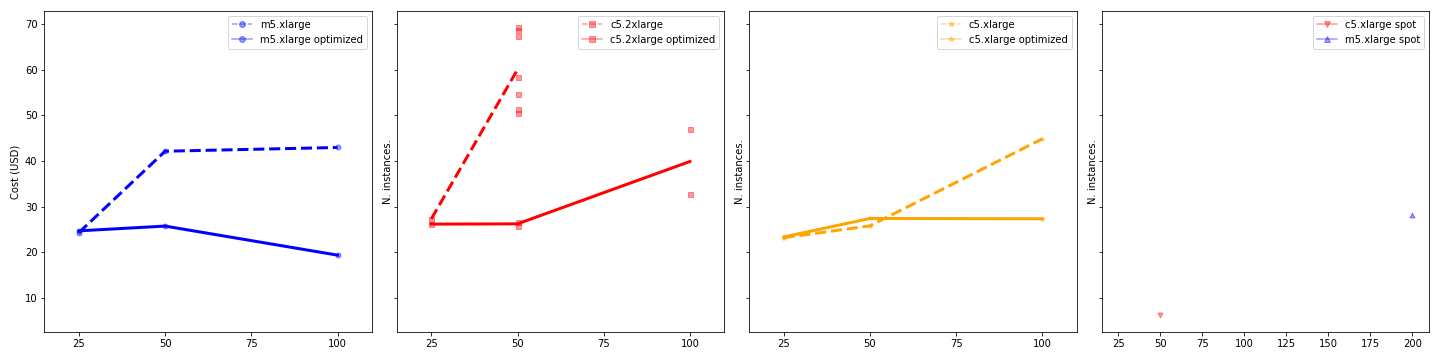
\includegraphics[width=\columnwidth]{figures/Cost.png}
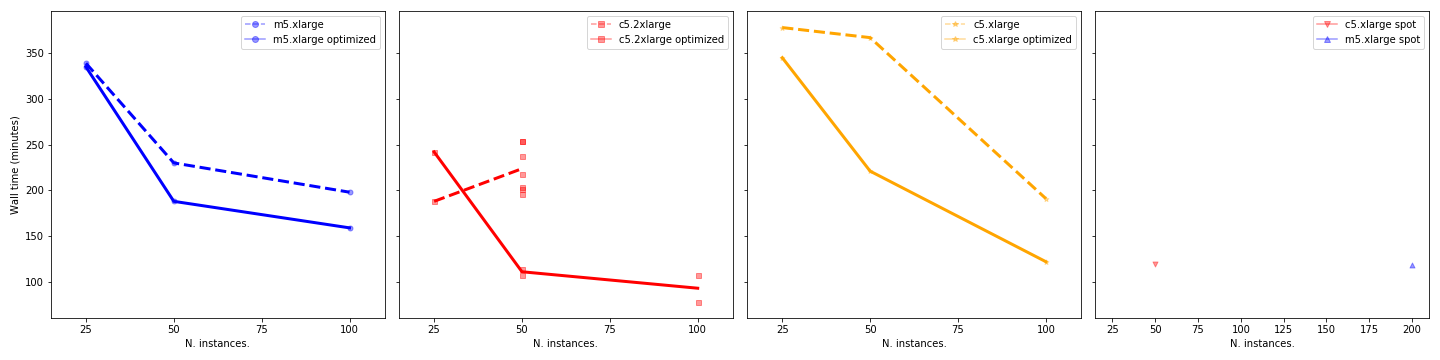
\includegraphics[width=\columnwidth]{figures/WallTime.png}
\caption{Top figure shows the total wall time versus number of workers used to execute the workflow for non-optimal test runs (dashed) and optimal (full line) test workflow executions. The optimal workflows almost always run faster than the non-optimal ones. The case of c5.2xlarge optimal run with 25 instances taking longer than the non-optimal was an error with annex deallocation so the walltime is easily overestimated by a factor of 2. There are no non-optimal c5.2xlarge tests because the cluster is under-subscribed and workers are automatically deallocated quickly leading to a cluster with approximately 50 instances. \\
The top figure shows Cost versus number of instances for the same setup. Figure shows how cost optimization can be non-intuitive function of requirements of workflow Quanta, cluster and scheduler configurations. Running workflow on clusters with more vCPUs can lead to  no additional cost, or even a slight reduction in cost, when the cluster is oversubscribed because the walltime is decreased significantly. For c5.2xlarge clusters price approximately scales with the number of instances, i.e. it costs more but is quicker, because in those scenarios we were not over or undersubscribed to the same extent as in others. Renting 200 m5.xlarge spot instances, right-most, shows that scaling can be achieved at reasonable prices. Since the number of vCPUs is the same as tests with 50 c5.2xlarge tests the timings and the cost are approximately the same. Maximal savings are achieved when optimal case scenario, 50 c5.2xlarge instnaces, are run using spot instances.}
\label{fig:demo-workflow}
\end{figure}


%\begin{table*}[t]
%\centering
%    \begin{tabular}{c c c c c c }
%    Run name  & Instance count & Cost & Wall Time & Comment \\
%    \hline \\
%    \multicolumn{5}{c}{m5.xlarge} \\
%    \hline \\
%    \rowcolor{lightgray}
%    20200116T213148  & 25  & 24.34  & 5h39m & - \\
%    \rowcolor{lightgray}                        
%    20200115T172359  & 50  & 42.15  & 3h50m & - \\
%    \rowcolor{lightgray}                        
%    20200116T175704  & 100 & 42.97  & 3h18m & - \\
%    20200309T135739  & 25  & 24.72  & 5h35m & - \\
%    20200309T194101  & 50  & 25.76  & 3h8m  & - \\
%    20200309T225436  & 100 & 19.40  & 2h39m & Compute resources not allocated %for 32m43s after scheduling the jobs.\\
%    \hline \\                                                 
%    \multicolumn{5}{c}{c5.2xlarge} \\
%    \hline \\
%    \rowcolor{lightgray}                                        
%    20200127T010224  & 25  & 27.33  & 3h8m  & - \\
%    \rowcolor{lightgray}                         
%    20200127T162240  & 50  & 50.45  & 3h16m & - \\
%    \rowcolor{lightgray}                         
%    20200128T192127  & 50  & 67.48  & 3h38m & - \\
%    \rowcolor{lightgray}                         
%    20200128T234142  & 50  & 54.62  & 3h58m & - \\
%    \rowcolor{lightgray}                         
%    20200129T034251  & 50  & 68.59  & 4h14m & - \\
%    \rowcolor{lightgray}                         
%    20200129T184318  & 50  & 51.34  & 3h22m & Replenished burst balance. \\
%    \rowcolor{lightgray}                         
%    20200129T221952  & 50  & 58.47  & 3h24m & Replenished burst balance.  \\
%    \rowcolor{lightgray}                        
%    20200130T021620  & 50  & 69.28  & 4h14m &  -  \\
%    20200302T222936  & 25  & 26.19  & 4h2m  & Wall time is wrong, job %forgotten. \\
%    20200227T232007  & 50  & 26.72  & 1h54m & - \\
%    20200228T014417  & 50  & 25.78  & 1h48m & Optimal cluster size. \\
%    20200302T180554  & 100 & 47.08  & 1h48m & Under-subscribed cluster. \\
%    20200302T210301  & 100 & 32.72  & 1h18m & A more appropriate cluster size %than 180553 but still not optimal. \\
%    \hline \\                
%    \multicolumn{5}{c}{c5.xlarge} \\                                
%    \hline \\
%    \rowcolor{lightgray}                               
%    20200123T165014  & 25  & 23.22  & 6h18m & Annex did not de-allocate %automatically accidentally restarted the master node. \\
%    \rowcolor{lightgray}                      
%    20200126T175516  & 50  & 25.81  & 6h7m  & - \\
%    \rowcolor{lightgray}                      
%    20200123T232152  & 100 & 44.86  & 3h11m & - \\
%    20200305T182023  & 25  & 23.38  & 5h45m & Potentially overestimated %pricing. \\ 
%    20200305T182023  & 50  & 27.43  & 3h41m & Forgotten run timings and cost %are overestimated. \\
%    20200306T062555  & 100 & 27.36  & 2h2m  & - \\
%    \hline \\
%    \multicolumn{5}{c}{Spot} \\                                     
%    \hline \\
%    20200310T191539  & 200 & 28.21 & 1h58m & Instance type and size: m5.large %\\
%    20200310T183810  & 50   & 6.24  & 1h59m & Instance type and size: %c5.2xlarge
%\end{tabular}
%\caption{Caption}
%\label{tbl:cost}
%\end{table*}






%\begin{table*}[t]
%\centering
%    \begin{tabular}{c c c c c c }
%    Run name  & Instance count & Cost & Wall Time & Comment \\
%    \hline \\
%    \multicolumn{5}{c}{m5.xlarge} \\
%    \hline \\
%    \rowcolor{lightgray}
%    20200116T213148  & 25  & 24.34  & 5h39m & - \\
%    \rowcolor{lightgray}                        
%    20200115T172359  & 50  & 42.15  & 3h50m & - \\
%    \rowcolor{lightgray}                        
%    20200116T175704  & 100 & 42.97  & 3h18m & - \\
%    20200309T135739  & 25  & 24.72  & 5h35m & - \\
%    20200309T194101  & 50  & 25.76  & 3h8m  & - \\
%    20200309T225436  & 100 & 19.40  & 2h39m & \specialcell{Compute resources not allocated for \\ 32m43s %after scheduling the jobs.}\\
%    \hline \\                                                 
%    \multicolumn{5}{c}{c5.2xlarge} \\
%    \hline \\
%    \rowcolor{lightgray}                                        
%    20200127T010224  & 25  & 27.33  & 3h8m  & - \\
%    \rowcolor{lightgray}                         
%    20200127T162240  & 50  & 50.45  & 3h16m & - \\
%    \rowcolor{lightgray}                         
%    20200128T192127  & 50  & 67.48  & 3h38m & - \\
%    \rowcolor{lightgray}                         
%    20200128T234142  & 50  & 54.62  & 3h58m & - \\
%    \rowcolor{lightgray}                         
%    20200129T034251  & 50  & 68.59  & 4h14m & - \\
%    \rowcolor{lightgray}                         
%    20200129T184318  & 50  & 51.34  & 3h22m & Replenished burst balance. \\
%    \rowcolor{lightgray}                         
%    20200129T221952  & 50  & 58.47  & 3h24m & Replenished burst balance.  \\
%    \rowcolor{lightgray}                        
%    20200130T021620  & 50  & 69.28  & 4h14m &  -  \\
%    20200302T222936  & 25  & 26.19  & 4h2m  & Wall time is wrong, job forgotten. \\
%    20200227T232007  & 50  & 26.72  & 1h54m & - \\
%    20200228T014417  & 50  & 25.78  & 1h48m & Optimal cluster size. \\
%    20200302T180554  & 100 & 47.08  & 1h48m & Under-subscribed cluster. \\
%    20200302T210301  & 100 & 32.72  & 1h18m & \specialcell{A more appropriate cluster size than 180553 \\ %but still not optimal.} \\
%    \hline \\                
%    \multicolumn{5}{c}{c5.xlarge} \\                                
%    \hline \\
%    \rowcolor{lightgray}                               
%    20200123T165014  & 25  & 23.22  & 6h18m & \specialcell{Annex did not de-allocate automatically \\ %accidentally restarted the master node.} \\
%    \rowcolor{lightgray}                      
%    20200126T175516  & 50  & 25.81  & 6h7m  & - \\
%    \rowcolor{lightgray}                      
%    20200123T232152  & 100 & 44.86  & 3h11m & - \\
%    20200305T182023  & 25  & 23.38  & 5h45m & Potentially overestimated pricing. \\ 
%    20200305T182023  & 50  & 27.43  & 3h41m & \specialcell{Forgotten run timings and cost \\ are %overestimated.} \\
%    20200306T062555  & 100 & 27.36  & 2h2m  & - \\
%    \hline \\
%    \multicolumn{5}{c}{Spot} \\                                     
%    \hline \\
%    20200310T191539  & 200 & 28.21 & 1h58m & Instance type and size: m5.large \\
%    20200310T183810  & 50   & 6.24  & 1h59m & Instance type and size: c5.2xlarge
%\end{tabular}
%\caption{Caption}
%\label{tbl:cost}
%\end{table*}





%\begin{table*}[t]
%\centering
%\begin{tabular}{c|c|c|c|c|c|c }
%Run name & Type and size & Instance count & Cost & Wall Time & Spot & Comment \\
%\hline 
%20200302T222936  & c5.2xlarge    & 25   & 26.19  & 4h2m   & No & Wall time is wrong. \\
%20200227T232007  & c5.2xlarge    & 50   & 26.72  & 1h54m  & No & - \\
%20200228T014417  & c5.2xlarge    & 50   & 25.78  & 1h48m  & No & Optimal cluster size. \\
%20200302T180554  & c5.2xlarge    & 100  & 47.08  & 1h48m  & No & Under-subscribed cluster. \\
%20200302T210301  & c5.2xlarge    & 100  & 32.72  & 1h18m  & No & \specialcell{Better than 10301, but still \\ not optimal cluster size} \\
%20200305T182023  & c5.xlarge     & 25   & 23.38  & 5h45m  & No & Overestimated pricing. \\ 
%20200305T182023  & c5.xlarge     & 50   & 27.43  & 3h41m  & No & Timings and cost slightly off. \\
%20200306T062555  & c5.xlarge     & 100  & 27.36  & 2h2m   & No & - \\
%20200309T135739  & m5.xlarge     & 25   & 24.72  & 5h35m  & No & - \\
%20200309T194101  & m5.xlarge     & 50   & 25.76  & 3h8m   & No & - \\
%20200309T225436  & m5.xlarge     & 100  & 19.40  & 2h39m  & No & \specialcell{Compute resources %accidentally not allocated for \\ 32m43s after the jobs got scheduled.}\\
%20200310T191539  & m5.large      & 200  & 28.21 & 1h58m   & Yes & - \\
%20200310T183810  & c5.2xlarge    & 50   & 6.24  & 1h59m   & Yes & - \\
%\end{tabular}
%\label{tbl:cost}
%\end{table*}

%%%%%%%%%%%%%%%%%%%%%%%%%%%%%%%%%%%%%%%%%%%%%%%%%%%%%%%%%%%%%%%%%%%%%%%%%%%%%%%%
\section{Results and Discussion}

In Figure ??? we show the relative performance of the baseline and optimized workflow.


First take the canonical approach and show a figure for the below 

left yaxis time and right y axis cost

x            x
x            x x
x x.         x x
on-demand.  spot

Then describe it in the text without saying jarring

 The most jarring comparison of the performance of the implementation were run 20200130T021620, which took 4 hours and 14 minutes and cost nearly 70\$ and run 20200228T014417 which took 1 hour and 54 minutes and cost just shy of 26\$. When the same workflow was executed on spot instances, instead of on-demand instances, the total cost was an entirety of 6.24\$.



Costing estimates were performed for a more encompassing workflow than the example workflow, it additionally included coaddition and coaddition source measurements, with the same dataset in \cite{dmtn137}. Naive runs of the workflow on AWS cost approximately 95\$ but the workflow cost is dominated by the various bottlenecks we identified in the example workflow as the larger workflow is not yet optimized in the same manner as the example workflow. Given that the further efforts in characterizing the workflow resource requirements and subsequent optimizations produce similar cost wall time reductions and cost decrease the cost for running the workflow on AWS would be in a much more comparative 38\$ to 57\$ range. On premise cost estimates are performed for Rubin observatory \cite{dmtn135} compute resources estimating 36\$ for a workflow run. 

Many changes were already made and incorporated into the code that mitigate many of the mentioned bottlenecks. 

In Figure ??? we show the performance and cost scaling tests. These show that the wall time of a workflow scales linearly with ...

Our performance and cost scaling tests indicate that the wall time of a workflow scales linearly with the number of vCPUs used. Therefore a test with 200 m5.large (400 vCPUs) instances finishes in the same walltime as a 50 c5.2xlarge instances (400 vCPUs). 
%This seems to match the performance observed by Rubin Obs test runs. 
The cost is, however, dramatically different. The wall-clock  is a function of instance type and instance size, which is in turn constrained by the task resource requirements. 


Show 2 figures with just m5.xlarge  and c5.xlarge. One is cost and the other wall clock as a bar graph so it looks like

x            x              x
x            x              xx
x            x x            xx
x x          x x            xxx
25           50             100

where the x's are m5.xlarge, m5.xlarge(optimized), c5.xlarge, c5.xlarge(optimized), 

For the 50 add one more column for spot and use this as an example of spot cost saving



In general the scaling performance does not seem to be limited by IO or connection bandwidth on the workers mainly due to the distributive properties of S3 for typical file sizes in the Science Pipelines. The upper limit is generally set by the size of the instance that hosts the Registry. While scaling out to many workers seems to work, since all jobs need to contact the registry, there is an actual upper limit to the number of workers one might execute on simultaneously. This limit is set by the maximum number of simultaneous connections, and maximum allowed number of locks per connection, that are in turn dependant on the available cache size of the RDS instance. The largest RDS instance available is the db.m5.24xlarge with 96 vCPUs, 384GB of memory and 14000 Mbps of write speed to the attached EBS drives but the associated costs of such on-demand setup soon become prohibitive, with estimated monthly cost of nearly 12500\$. 

In a setup where this functionality is offered as a service, however, it is possible to significantly amortize these costs by procuring reserved instances instead. In that case it is possible to achieve 40\% discount by reserving such an instance for a year, 60\% for three years and it is also possible to negotiate pricing for longer reservation times with AWS directly. Similar savings can be achieved for master, or indeed any other persistent, instances as well. 

%We identify two major obstacles to adoption of such a system: difficulty of use, including both the significant amount of initial familiarization with novelty cloud services and perceived dificult-ness {\color{red} andy please help with this sentence} of running and managing the workflow and resources. 

%%%%%%%%%%%%%%%%%%%%%%%%%%%%%%%%%%%%%%%%%%%%%%%%%%%%%%%%%%%%%%%%%%%%%%%%%%%%%%%%
\section{Conclusions}

Optimizing costs for a general Quantum Graph is very challenging because the cost is mainly the function of wall-clock offset by the approximately constant cost of the RDS instance and monotonically growing S3 storage. 


I think the key messages are:
1. You can run legacy code on cloud
2. Looking at the IO can improve the performance by X
3. Looking at the cost and run time we can optimize based on instance type and this means that for our case you should use ? if you have a fixed budget and ? if you want to minimize time.

Making this information available to the user prior to launching a job is critical for any science gateway


It is crucial the have a very good characterization of each individual task requirements to be able to allocate resources in the most optimal manner. This however is hindered by the fact that resource allocation is not yet easily handled in a dynamical manner where users could adopt a submit-and-forget style of data processing. Adding more fine grained control, possibly defined in the Quantum Graph itself, that would allow for launching or targeting job execution to particular resources tailored specifically to that type of job would be a great improvement to the current workflow and resource management system in this context.

We motivate a use case for a gateway to astronomical data science processing in the cloud based on the ever growing data volumes produced by new astronomical sky surveys and the standardization of astronomical image processing. We propose a design for the backend to one such gateway based on the LSST Science Pipelines by utilizing Pegasus WMS as a workflow manager and HTCondor, and condor\_annex, as the resource manager. We demonstrated that performance and costing are not significantly impacted by the transition to the cloud. We also stress the importance of well characterized workflows and the impact that has on both performance and costing. We describe how it is possible to optimize sets of similar tasks in the workflow and identify missing functionality that would enable easier use of the proposed gateway. We additionally identify and briefly discuss, Jupyter Notebook a potential front-end interface choices given it's wide adoption within Astronomy. 



%%%%%%%%%%%%%%%%%%%%%%%%%%%%%%%%%%%%%%%%%%%%%%%%%%%%%%%%%%%%%%%%%%%%%%%%%%%%%%%%

\bibliographystyle{ieeetr}
\bibliography{bibliography}
\section{Acknowledgements}
\noindent We would like to that Rubin Observatory and the AWS PoC group which were instrumental in testing and eventually adopting and committing to maintaining much of the code written that was required to facilitate AWS processing. 
\clearpage
\end{document}
